\documentclass[10pt,letterpaper]{article}
\usepackage{amsmath,amssymb,geometry,graphicx}
\usepackage{enumitem}
%\settextfont{B Nazanin}
\usepackage{lipsum}
\setlength{\parskip}{3mm}
\setlength{\parindent}{0mm}
\newcommand{\wid}{0.49\textwidth}
\newcommand{\widone}{60mm}
\begin{document}
\Large
\begin{center}
In the name of beauty

9th problem set of ComNet course

\hrulefill
\end{center}
Q1) Determine the following statements as true or false. (Use enough reasons and explanation to support your answer)

\begin{enumerate}[label=\alph*-]
\item
Forward error correction (FEC) is the ability of error detection at the receiver.
\item
TDMA and FDMA are two prominent types of random access protocols for dividing the transmission media equally among all the users.
\item
Slotted ALOHA requires synchronization among users while ALOHA can be implemented totally distributedly.
\item
In ARP process, a user who joins a LAN starts by sending frames which have the MAC address of the local switch in their destination MAC address.
\end{enumerate}

Q2) Describe the steps of sending packets in all the data link to application layers  from when a user joins a LAN until it is assigned an IP address through DHCP. After its IP address is assigned, how does it know the MAC address of the interface of the first-hop router to insert in the destination field of the frames?

Q3) 
Consider slotted ALOHA for multiple access transmission. Assume that each node starts transmitting with probability $p$ at each time slot and there are $N$ nodes in total. Each frame exactly fits to each time slot (i.e. $F=R\times T$ where $F$, $R$ and $T$ are frame length, link capacity and time slot length, respectively). How many times (i.e. at how many time slots), in average, should a node send a frame in consecutive time slots to make sure the frame has been correctly received? Does the derived formula contain an optimum as a function of $p$? If so, find it and if not, explain why.

Q4) In the following network, assume the red squares be layer-2 switches and the green circles as hosts (the tiny numbers denote the interface IDs. Also the switches S1 and S4 are connected through a wireless connection):
\begin{center}
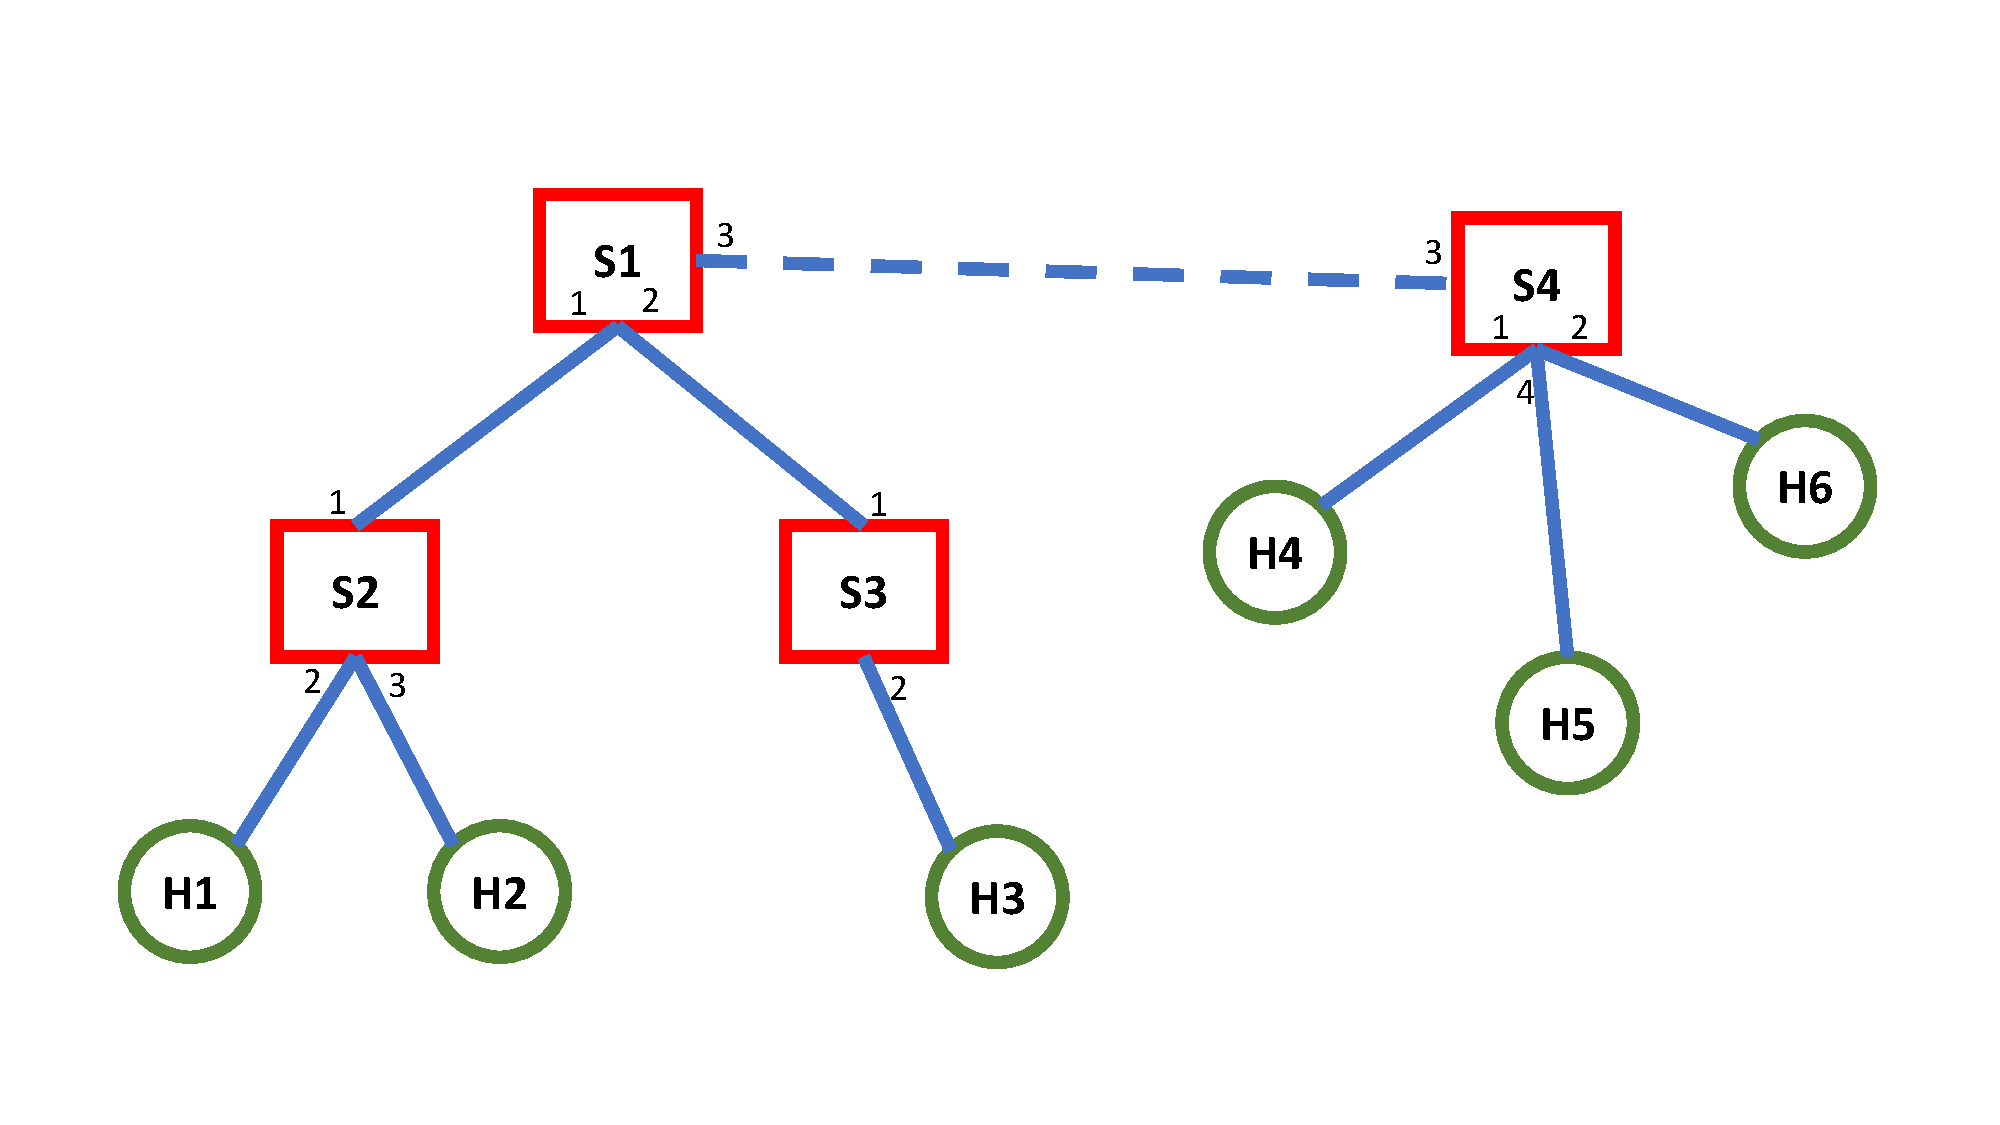
\includegraphics[width=120mm]{Q5_HW8}
\end{center}
a) What information is stored in all the switches when the host H1 with MAC address AA:AA:AA:AA:AA:AA broadcasts a frame considering the self-learning phase? (Drop the TTL arbitrarily in this part)

b) Assume that the host H3 wants to send a packet to H6 while the information of H6 are not recorded in S4 switch table. Where does the switch S4 forward the upstream packet?

Q5) Consider the single switch VLAN in Figure 5.25, and assume an external
router is connected to switch port 1. Assign IP addresses to the EE and CS
hosts and router interface. Trace the steps taken at both the network layer and the link layer to transfer an IP datagram from an EE host to a CS host (Hint: reread the discussion of Figure 5.19 in the textbook).
\end{document}